\documentclass{bioinfo}
\copyrightyear{2015} \pubyear{2015}

\access{Advance Access Publication Date: Day Month Year}
\appnotes{Manuscript Category}

\usepackage{bm}
\newcommand{\xmat}{{\bm X}}
\newcommand{\xref}{{\bm X}^{\mbox{ref}}}



\begin{document}
\firstpage{1}

\subtitle{Subject Section}

\title[Sample-specific co-expression networks]{Sample-specific co-expression networks}
\author[Azencott]{Chlo\'e-Agathe Azencott\,$^{\text{\sfb 1, 2, 3}*}$}
\address{$^{\text{\sf 1}}$MINES ParisTech, PSL-Research University, CBIO-Centre for Computational Biology, 35 rue St Honor\'e 77300 Fontainebleau, France\\
$^{\text{\sf 2}}$Institut Curie, 75248 Paris Cedex 05, France\\
$^{\text{\sf 3}}$INSERM, U900, 75248 Paris Cedex 05, France}

\corresp{$^\ast$To whom correspondence should be addressed.}

\history{Received on XXXXX; revised on XXXXX; accepted on XXXXX}

\editor{Associate Editor: XXXXXXX}

\abstract{\textbf{Motivation:} \\
\textbf{Results:} \\
\textbf{Availability:} Code is available at \href{https://github.com/chagaz/SamSpecCoEN}{https://github.com/chagaz/SamSpecCoEN}\\
\textbf{Contact:} \href{chloe-agathe.azencott@mines-paristech.fr}{chloe-agathe.azencott@mines-paristech.fr}\\
\textbf{Supplementary information:} Supplementary data are available at \textit{Bioinformatics}
online.}

\maketitle

\section{Introduction}

Co-expression networks are a powerful and much used tool to analyze and visualize gene-expression data at a population level. 
They can be used to contrast two populations, for example healthy vs. diseased. 
They represent the correlation between genes.
Once they have been computed, samples can be represented by mapping their individual gene expression levels to the nodes of the network: the network structure is set once and for all, and the samples differ by their node weights.

What we propose here is to define patient-specific networks, in which the samples differ by their edge weights. We have two goals in mind: a different way of representing the data might lead to new insights. In addition, different learning algorithms can be applied to data where instances are represented as different networks. To the best of our knowledge, this has only been proposed once before~\citep{kuijjer2015}.





%\enlargethispage{12pt}

\section{Approach}

We propose to build sample-specific gene co-expression networks from traditional gene co-expression networks, by assigning different weights to their edges for different patients. These weights quantify how much the sample deviates from the population for this particular gene-gene association. 

\begin{figure}[!tpb]
  % \fboxsep=0pt\colorbox{gray}{\begin{minipage}[t]{235pt} \vbox to 100pt{\vfill\hbox to
  %       235pt{\hfill\fontsize{24pt}{24pt}\selectfont FPO\hfill}\vfill}
  %   \end{minipage}}
  \centerline{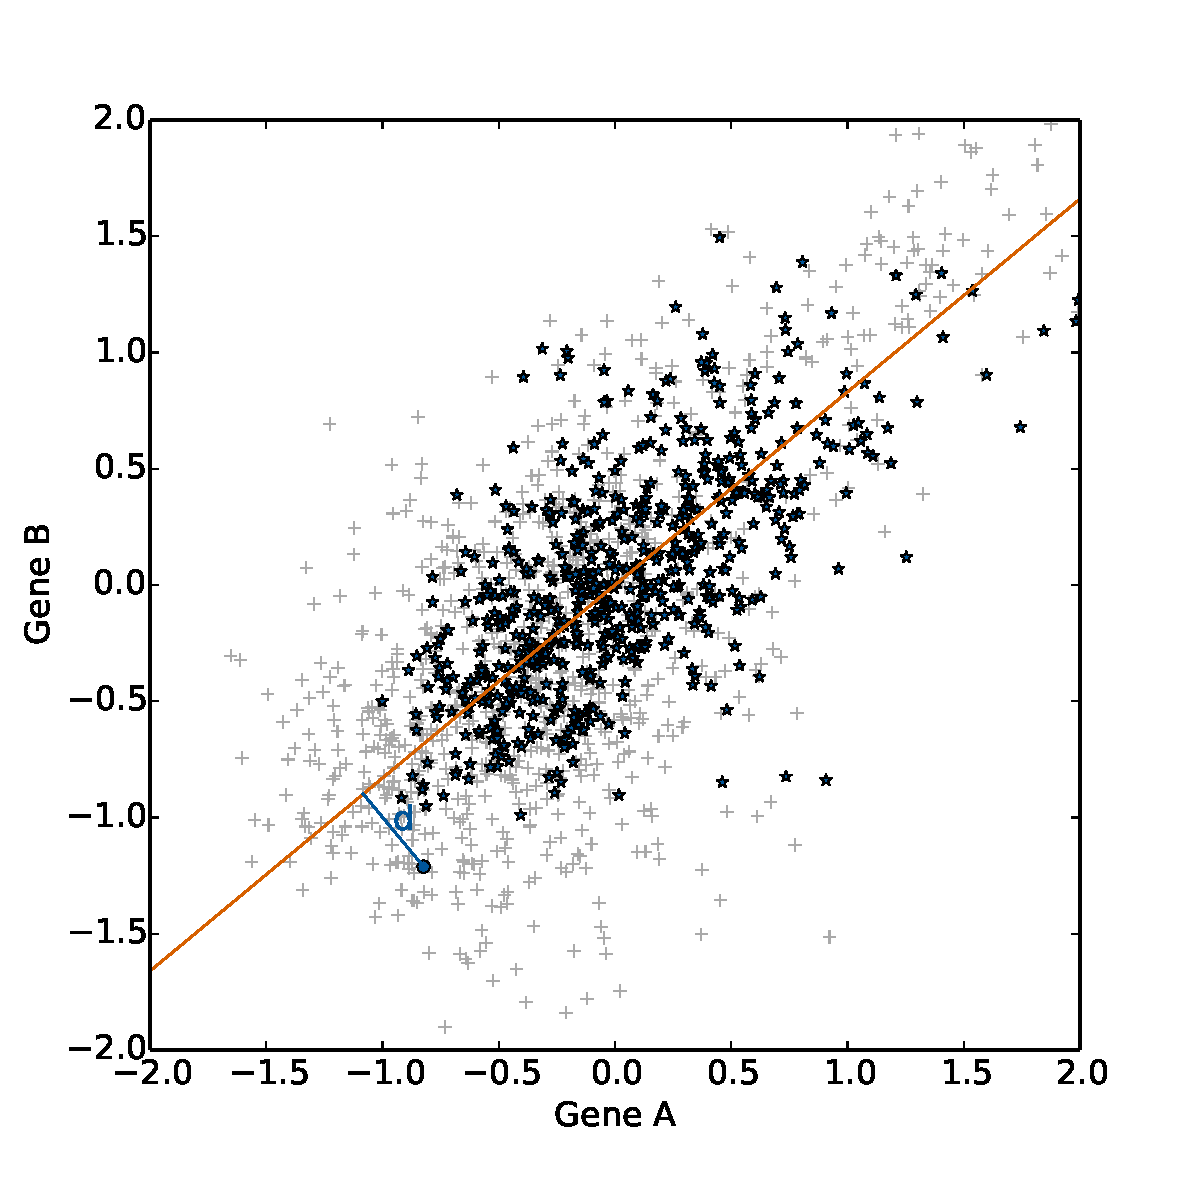
\includegraphics[width=0.5\textwidth]{regline_example.pdf}}
  \caption{Distance to the regression line of Gene B against Gene A represents how much a patient ``deviates from the norm'', for the (A, B) co-expression pattern. Gray crosses represent reference samples; blue stars represent data samples; the orange line is the regression line of Gene B against Gene A for the reference samples; 'd' is the distance to the regression line of a specific sample, represented by a blue cirle.}
  \label{fig:distance_to_regline}
\end{figure}



\begin{methods}
\section{Methods}
Let us assume $n$ samples, $p$ genes, the expression $\xmat \in \mathbb{R}^{n \times p}$ of these $p$ genes in the $n$ samples, the binary outcome $Y \in \{0, 1\}^n$ for the $n$ samples.
Let us further assume a reference data set of $N$ samples and the same $p$ genes, with expression $\xref \in \mathbb{R}^{N \times p}$.





\subsection{Population-wide gene co-expression networks}

\subsection{Sample-specific edge weights}

\subsubsection{LIONESS}
~\citealp{kuijjer2015} propose to.

LIONESS~\cite{kuijjer2015} is, to the best of our knowledge, the only existing method to build sample-specific co-expression networks from gene expression data.\\

LIONESS considers that the global network is made of the aggregation of individual contributions from each sample. 
Denoting by $e_{ij}^\alpha$ the weight of the edge between $i$ and $j$ computed over all samples;
by $e_{ij}^{(\alpha - q)}$ the weight of the edge between $i$ and $j$ computed over all samples but sample $q$;
and by $e_{ij}^q$ the weight of the edge between $i$ and $j$ contributed by sample $q$:
    \[
    e_{ij}^\alpha = \sum_{s=1}^n \frac{1}{n} e_{ij}^s 
    \mbox{ and }
    e_{ij}^{(\alpha - q)} = \sum_{s=1}^n \frac{1}{(n-1)} e_{ij}^s
    \]

Hence
    \[
    e_{ij}^q = \frac{1}{n} \left(  e_{ij}^{\alpha} - e_{ij}^{(\alpha - q)} \right) + e_{ij}^{(\alpha - q)}.
    \]

In the case of a network computed using Pearson's correlation, assuming the number $n$ of samples to be large,~\cite{kuijjer2015} show that the individual contributions of each sample can be approximated by
    \[
    e_{ij}^q \approx \frac{n}{n-1} \left( \frac{\xmat_i^q - \bar {\xmat_i}}{S_{\xmat_i}} \right) 
    \left( \frac{\xmat_j^q - \bar {\xmat_j}}{S_{\xmat_j}} \right)
    \]
    where $S_{\xmat_i} = \sqrt{\frac{1}{n-1} \sum_{s=1}^n \left( \xmat_i^s - \bar{\xmat_i} \right)^2}$ is the sample standard deviation of gene $i$.



\subsubsection{REGLINE}
Also based on Pearson's correlation, we propose to compute sample-specific edge weights based not on the contribution of each sample to the total correlation, but on the deviation of each sample from the overall relationship between both genes. To this aim, we use the distance of the sample to the regression line between both variables.

A major difference with LIONESS is that we compute this overall relationship, or regression line, over the {\em reference} data.

Given a pair $(i, j)$ of genes, we fit a regression line $\beta_0^{ij} + \beta_1^{ij} \xref_i = \xref_j$, and the edge weight of $(i, j)$ for sample $q$ is given by:

\[
e_{ij}^q = \frac{|\beta_1^{ij} x_i - x_j + \beta_0^{ij}|}{\sqrt{(\beta_1^{ij})^2+1}}.
\]


\subsection{Learning from sample-specific co-expression networks}

\subsubsection{Data}

\subsubsection{Validation framework}

\begin{figure}[!tpb]
  % \fboxsep=0pt\colorbox{gray}{ \begin{minipage}[t]{235pt} \vbox to 100pt{\vfill\hbox to
    %     235pt{\hfill\fontsize{24pt}{24pt}\selectfont FPO\hfill}\vfill}
    % \end{minipage}}
  \centerline{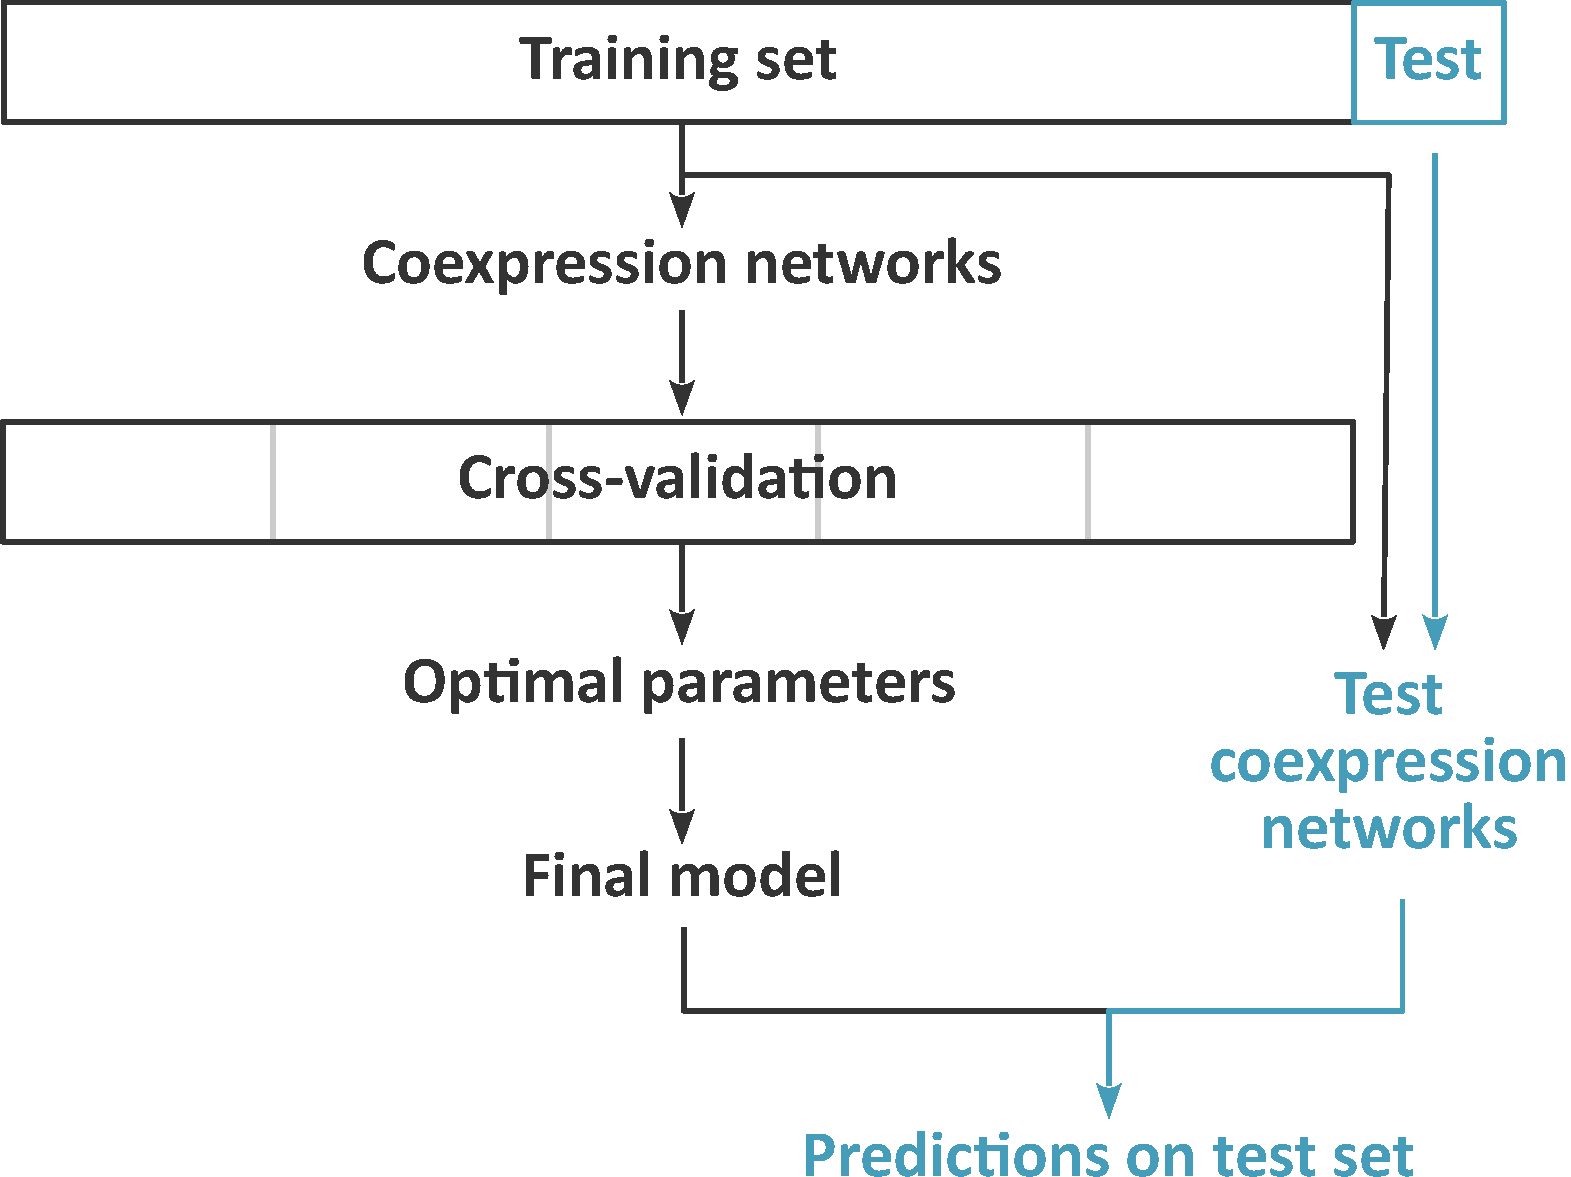
\includegraphics[width=0.4\textwidth]{eval_framework.pdf}}
  \caption{Nested cross-validation framework.}
  \label{fig:eval_framework}
\end{figure}



\subsubsection{Regularized logistic regression on edge weights}

\subsubsection{Comparison partners}
\begin{itemize}
\item l1-regularized logistic regression on node weights (gene expression)
\item l2-regularized logistic regression on connected node weights (gene expression)
\item l2-regularized logistic regression on a network-guided selection of nodes
\item FERAL~\cite{allahyar2015} is a state-of-the-art approach for network-based breast cancer outcome prediction from gene-expression profiles.\\
FERAL defines, for each $gene$ of a given biological network, a group of $10$ genes based on the neighborhood of this seed genes in the network. To each group, it adds $6$ non-linear meta-features, such as its average, median, or max gene expression. Finally, a Sparse Group Lasso classifier~\cite{friedman2010} is trained:
  \[
  \min_{\beta \in \mathbb{R}^d} \left( \ell(Y, \tilde \xmat  \beta) + \lambda_1 || \beta||_1 + 
  \lambda_2 \sum_{g=1}^G \sqrt{p_g}\, ||\beta_g||_2 \right),
  \]
  where $p_g = 16$ is the size of group $g$, 
  $\beta_g$ is the weight vector $\beta$ restricted to the indices 
  corresponding to the features in group $g$, 
  $\tilde \xmat$ is $\xmat$ augmented with the meta-features,
  and $\ell$ is the logistic loss function.

\end{itemize}




\enlargethispage{6pt}


% \begin{table}[!t]
% \processtable{This is table caption\label{Tab:01}} {\begin{tabular}{@{}llll@{}}\toprule head1 &
% head2 & head3 & head4\\\midrule
% row1 & row1 & row1 & row1\\
% row2 & row2 & row2 & row2\\
% row3 & row3 & row3 & row3\\
% row4 & row4 & row4 & row4\\\botrule
% \end{tabular}}{This is a footnote}
% \end{table}

\end{methods}

% \begin{figure}[!tpb]%figure1
% \fboxsep=0pt\colorbox{gray}{\begin{minipage}[t]{235pt} \vbox to 100pt{\vfill\hbox to
% 235pt{\hfill\fontsize{24pt}{24pt}\selectfont FPO\hfill}\vfill}
% \end{minipage}}
% %\centerline{\includegraphics{fig01.eps}}
% \caption{Caption, caption.}\label{fig:01}
% \end{figure}

%\begin{figure}[!tpb]%figure2
%%\centerline{\includegraphics{fig02.eps}}
%\caption{Caption, caption.}\label{fig:02}
%\end{figure}


%\subsection{Test1}




\section{Results}





%%%%%%%%%%%%%%%%%%%%%%%%%%%%%%%%%%%%%%%%%%%%%%%%%%%%%%%%%%%%%%%%%%%%%%%%%%%%%%%%%%%%%
%
%     please remove the " % " symbol from \centerline{\includegraphics{fig01.eps}}
%     as it may ignore the figures.
%
%%%%%%%%%%%%%%%%%%%%%%%%%%%%%%%%%%%%%%%%%%%%%%%%%%%%%%%%%%%%%%%%%%%%%%%%%%%%%%%%%%%%%%






\section{Discussion and Conclusion}


\section*{Acknowledgements}

Text Text Text Text Text Text  Text Text. \vspace*{-12pt}

\section*{Funding}

This work has been supported by the... Text Text  Text Text.\vspace*{-12pt}

\bibliographystyle{natbib}
%\bibliographystyle{achemnat}
%\bibliographystyle{plainnat}
%\bibliographystyle{abbrv}
%\bibliographystyle{bioinformatics}
%
%\bibliographystyle{plain}
%
\bibliography{../references}


% \begin{thebibliography}{}

% \bibitem[Bofelli {\it et~al}., 2000]{Boffelli03}
% Bofelli,F., Name2, Name3 (2003) Article title, {\it Journal Name}, {\bf 199}, 133-154.

% \bibitem[Bag {\it et~al}., 2001]{Bag01}
% Bag,M., Name2, Name3 (2001) Article title, {\it Journal Name}, {\bf 99}, 33-54.

% \bibitem[Yoo \textit{et~al}., 2003]{Yoo03}
% Yoo,M.S. \textit{et~al}. (2003) Oxidative stress regulated genes
% in nigral dopaminergic neurnol cell: correlation with the known
% pathology in Parkinson's disease. \textit{Brain Res. Mol. Brain
% Res.}, \textbf{110}(Suppl. 1), 76--84.

% \bibitem[Lehmann, 1986]{Leh86}
% Lehmann,E.L. (1986) Chapter title. \textit{Book Title}. Vol.~1, 2nd edn. Springer-Verlag, New York.

% \bibitem[Crenshaw and Jones, 2003]{Cre03}
% Crenshaw, B.,III, and Jones, W.B.,Jr (2003) The future of clinical
% cancer management: one tumor, one chip. \textit{Bioinformatics},
% doi:10.1093/bioinformatics/btn000.

% \bibitem[Auhtor \textit{et~al}. (2000)]{Aut00}
% Auhtor,A.B. \textit{et~al}. (2000) Chapter title. In Smith, A.C.
% (ed.), \textit{Book Title}, 2nd edn. Publisher, Location, Vol. 1, pp.
% ???--???.

% \bibitem[Bardet, 1920]{Bar20}
% Bardet, G. (1920) Sur un syndrome d'obesite infantile avec
% polydactylie et retinite pigmentaire (contribution a l'etude des
% formes cliniques de l'obesite hypophysaire). PhD Thesis, name of
% institution, Paris, France.

%\end{thebibliography}
\end{document}
